\chapter{Proposed System Architecture}\label{ch:arch}

Every component described in this chapter is present in the firmware. Nothing is included
because it would make the architecture look more complete, and where a component is absent that
a reader might expect, the absence is stated.

\section{Overview}

The architecture rests on one decision: the safety function and all network activity are placed
on separate cores and share nothing but three explicitly bounded objects. Figure~\ref{fig:arch}
shows the whole system.

\begin{figure}[htbp]
\centering
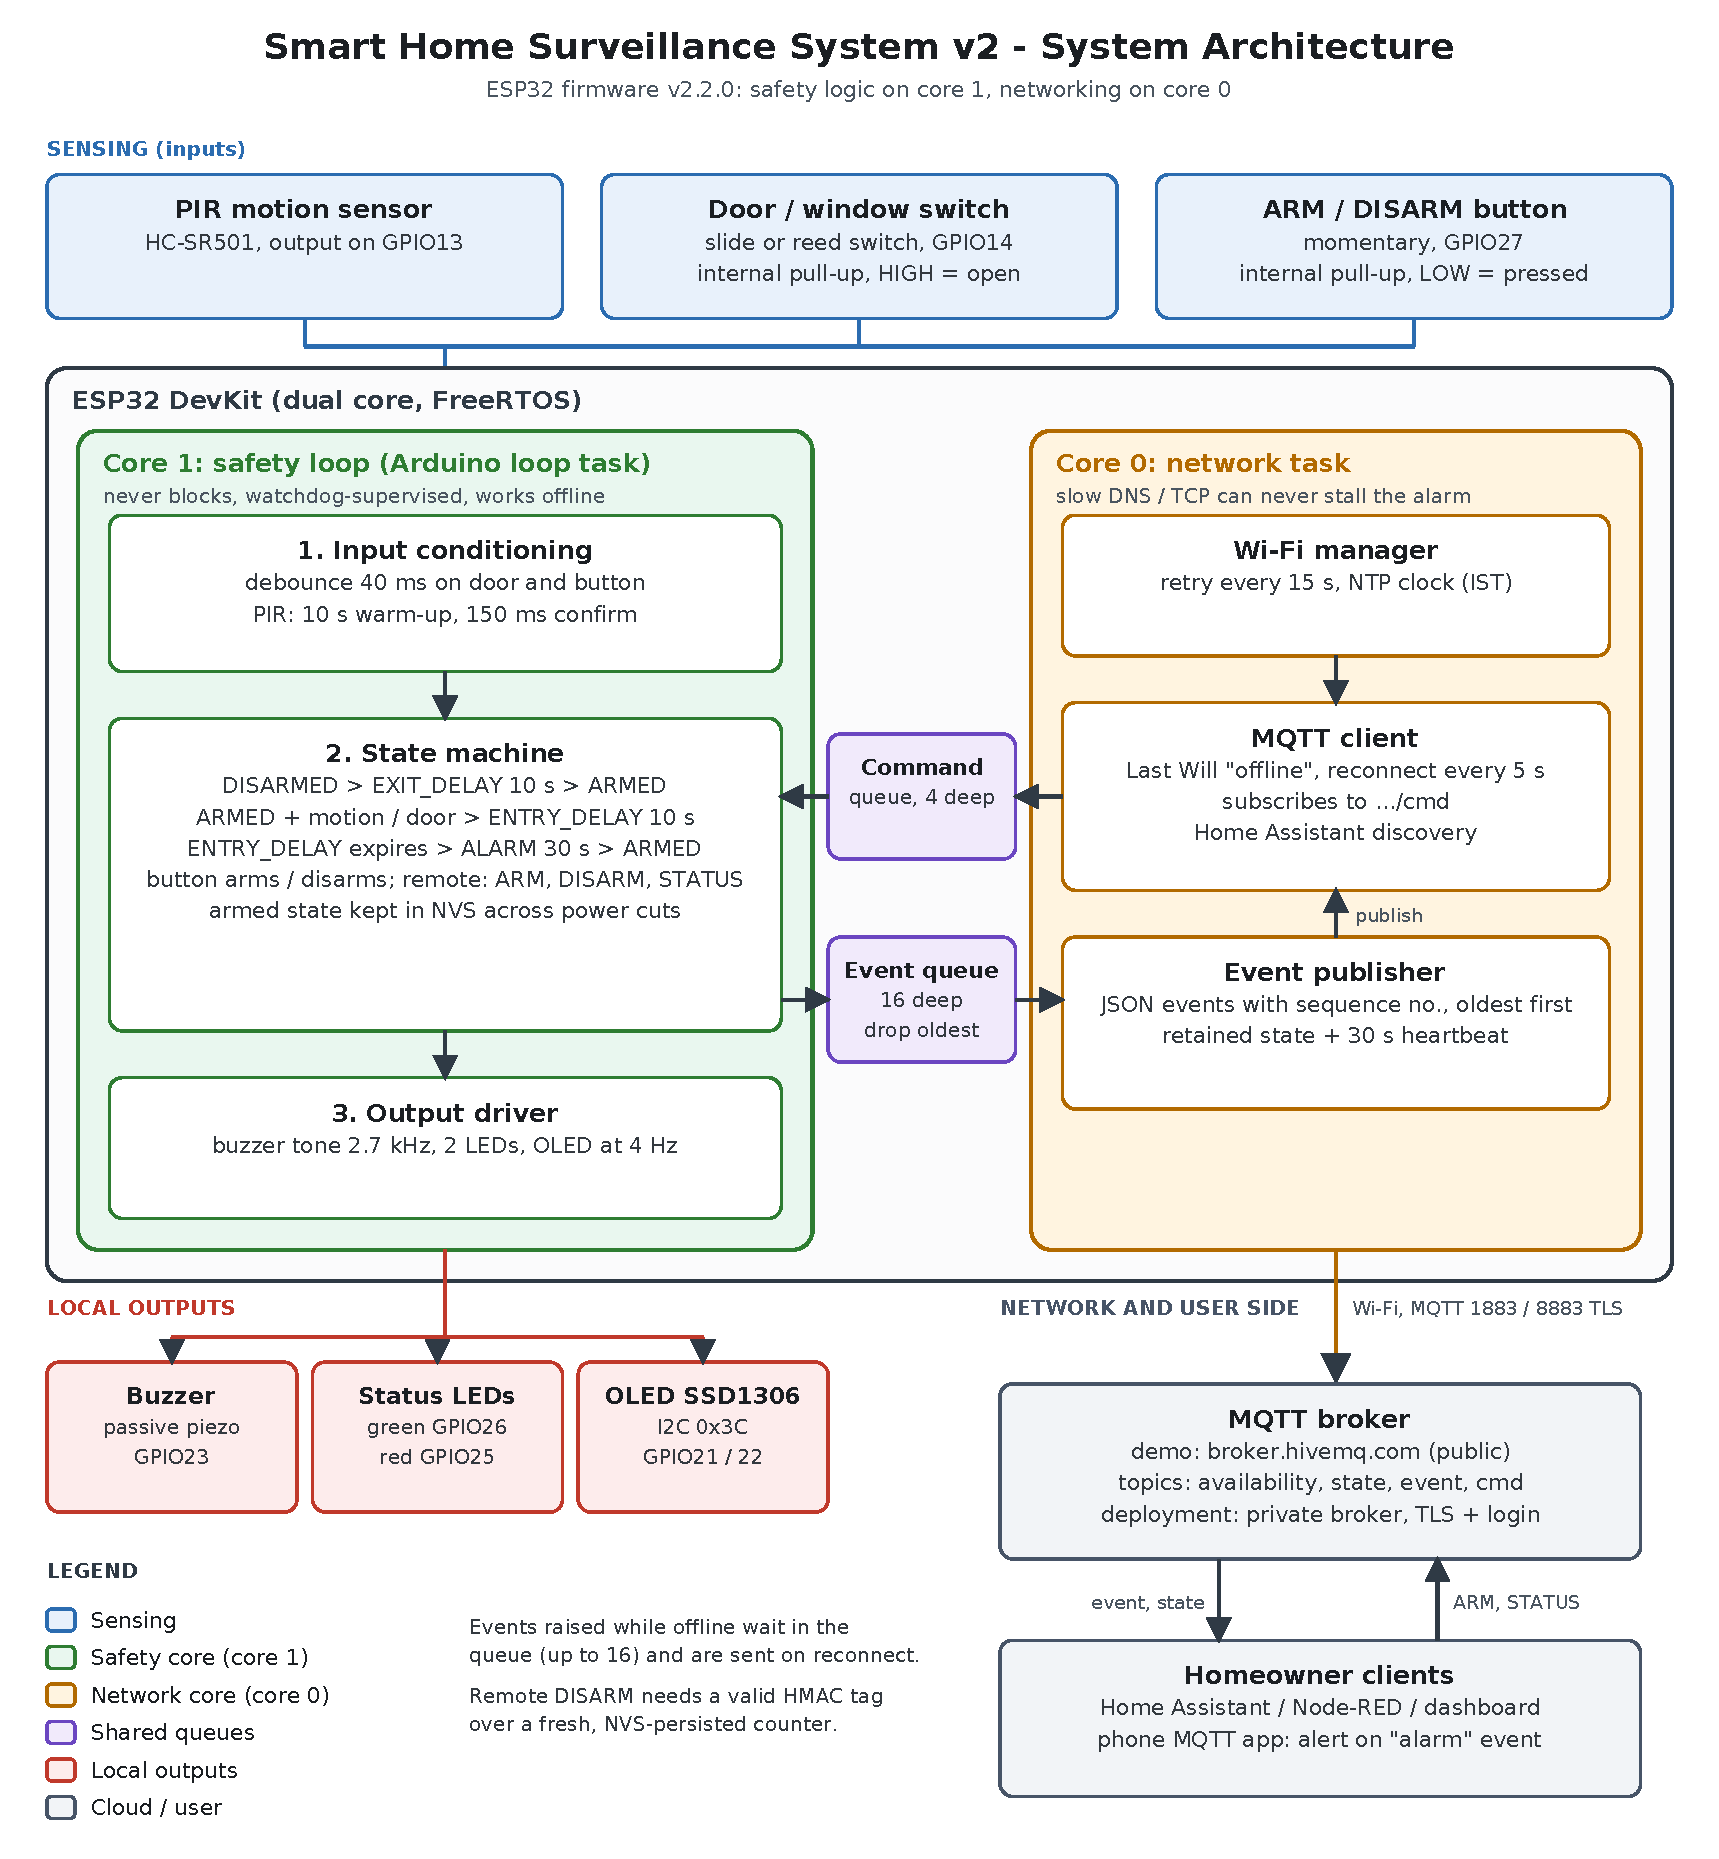
\includegraphics[width=0.96\textwidth,height=0.78\textheight,keepaspectratio]{architecture.pdf}
\caption[System architecture]{System architecture. The safety domain on core~1 (green) and the
network domain on core~0 (blue) communicate only through two bounded queues and one
mutex-guarded status snapshot. Every pin number, timeout and queue depth shown is transcribed
from \code{firmware/smart\_home/smart\_home.ino}.}
\label{fig:arch}
\end{figure}

\section{Hardware platform}

The device is an ESP32-WROOM-32 development board. The relevant properties are that it is
dual-core — two Xtensa LX6 cores — and that its 802.11 radio shares the die with them. A
single-core variant such as the ESP32-C3 cannot host this architecture at all, which is why
Appendix~\ref{app:hardware} insists on the dual-core part for the measurement.

\begin{longtable}{@{}p{0.22\textwidth}p{0.13\textwidth}p{0.57\textwidth}@{}}
\toprule
\textbf{Peripheral} & \textbf{Pin} & \textbf{Role} \\
\midrule
\endhead
PIR motion sensor (HC-SR501)  & GPIO 13 & Primary intrusion detector; 10\,s warm-up and a
150\,ms confirmation window \\
Door or window switch         & GPIO 14 & Reed or slide switch, internal pull-up, HIGH when
open \\
Arm/disarm button             & GPIO 27 & Momentary, internal pull-up, LOW when pressed,
40\,ms debounce \\
Siren (passive piezo)         & GPIO 23 & Driven at 2.7\,kHz \\
Armed indicator               & GPIO 26 & Green \\
Alarm indicator               & GPIO 25 & Red \\
OLED display (SSD1306)        & GPIO 21, 22 & I2C at address \code{0x3C}, refreshed every
250\,ms \\
\bottomrule
\end{longtable}

\section{Core 1: the safety domain}

Core 1 hosts the Arduino \code{loop()} task, which is the safety function. It performs three
stages in sequence on every pass.

\begin{enumerate}[leftmargin=1.8em,itemsep=4pt]
  \item \textbf{Input conditioning.} Sensor lines are sampled and debounced. The PIR is
        suppressed for 10\,s after power-up, because the HC-SR501 produces spurious output
        while stabilising, and a motion indication must persist for 150\,ms before it is
        treated as real.
  \item \textbf{State machine.} The conditioned inputs and any dequeued command advance a
        five-state machine. The armed state is written to non-volatile storage so that a power
        interruption does not disarm the system.
  \item \textbf{Output driver.} The siren, the two indicators and the display are driven from
        the current state.
\end{enumerate}

Two properties of this loop matter more than its contents. It \emph{never blocks}: every
acquisition of a shared resource uses a zero timeout and proceeds without it on failure. And it
is \emph{independent of the network}: with the radio disabled, every function in
Section~\ref{ch:req}'s FR1 to FR6 still works.

\subsection{The state machine}

\begin{longtable}{@{}p{0.17\textwidth}p{0.13\textwidth}p{0.62\textwidth}@{}}
\toprule
\textbf{State} & \textbf{Duration} & \textbf{Meaning and exits} \\
\midrule
\endhead
\code{DISARMED}    & ---     & Sensors are ignored. Exits on a local button press or an
authenticated \code{ARM}/\code{ARM\_AWAY}. \\
\code{EXIT\_DELAY} & 10\,s   & The occupant is leaving. Exits to \code{ARMED} on expiry. \\
\code{ARMED}       & ---     & Sensors are live. Motion or a door opening moves to
\code{ENTRY\_DELAY}. \\
\code{ENTRY\_DELAY}& 10\,s   & Grace period for a legitimate entry. A disarm here returns to
\code{DISARMED}; expiry moves to \code{ALARM}. \\
\code{ALARM}       & 30\,s   & The siren sounds. Returns to \code{ARMED} on expiry. \\
\bottomrule
\end{longtable}

\section{Core 0: the network domain}

Core 0 hosts a single FreeRTOS task created explicitly rather than by the framework:

\begin{lstlisting}[style=cpp,caption={Network task creation, \code{smart\_home.ino}},
                   label={lst:taskcreate}]
xTaskCreatePinnedToCore(networkTask, "net", 8192, nullptr, 1, nullptr, 0);
\end{lstlisting}

The final argument pins the task to core~0. The Arduino \code{loop()} runs on core~1 by
default, so the two domains are on separate cores without any further configuration. The task
performs Wi-Fi management, the MQTT client, and event publication.

\begin{itemize}[leftmargin=1.6em,itemsep=4pt]
  \item \textbf{Wi-Fi manager.} Reconnects every 15\,s on loss, and maintains an NTP-corrected
        clock for event timestamps.
  \item \textbf{MQTT client.} Reconnects every 5\,s, registers a Last Will message so the
        broker announces the device as offline, subscribes to the command topic and publishes
        Home Assistant discovery metadata.
  \item \textbf{Event publisher.} Publishes JSON events carrying a sequence number, oldest
        first, together with a retained state topic and a 30\,s heartbeat.
\end{itemize}

Every one of these operations can block for a long time. DNS resolution, TCP connection
establishment and the TLS handshake are all unbounded in the worst case. That is precisely why
they are on the other core.

\section{What the two domains share}

Exactly three objects cross the boundary, and the discipline applied to each is what the
isolation argument rests on.

\begin{longtable}{@{}p{0.20\textwidth}p{0.11\textwidth}p{0.61\textwidth}@{}}
\toprule
\textbf{Object} & \textbf{Bound} & \textbf{Discipline} \\
\midrule
\endhead
Command queue \code{cmdQ}  & 4 entries  & Core 0 enqueues non-blocking; core 1 drains at most
\code{CMD\_DRAIN\_PER\_PASS} entries per pass. \\
Event queue \code{eventQ}  & 16 entries & Core 1 enqueues non-blocking; the oldest entry is
dropped when full, so the safety loop never waits for a consumer. \\
Status snapshot            & 1 struct   & Guarded by \code{statusMutex}. Core 1 acquires with
timeout \textbf{0}; core 0 acquires with a 10\,ms timeout. Copied every 500\,ms. \\
\bottomrule
\end{longtable}

\subsection{The asymmetric mutex timeout}

The status snapshot is the mechanism most easily overlooked and it is the heart of the design.
Both cores need access to the same state structure: core~1 writes it, core~0 reads it in order
to publish. A conventional mutex would let the network core's acquisition delay the safety
core.

The firmware avoids this by making the timeouts asymmetric:

\begin{lstlisting}[style=cpp,caption={Asymmetric acquisition, \code{smart\_home.ino}},
                   label={lst:mutex}]
/* core 1, the safety loop: never waits */
if (xSemaphoreTake(statusMutex, 0) == pdTRUE) {
    /* copy the snapshot */
    xSemaphoreGive(statusMutex);
}
/* if the lock was unavailable, the loop simply continues; the snapshot
   is refreshed on the next pass 500 ms later */

/* core 0, the network task: may wait up to 10 ms */
if (xSemaphoreTake(statusMutex, pdMS_TO_TICKS(10)) == pdTRUE) {
    /* read the snapshot and publish */
    xSemaphoreGive(statusMutex);
}
\end{lstlisting}

The consequence is that the blocking term in the response-time analysis of
Section~\ref{sec:impl-rt} is \emph{identically zero by construction} rather than merely small.
The safety loop cannot be made to wait, because it never asks to. The cost is that a status
publication may occasionally carry a snapshot up to 500\,ms old, which is an acceptable price
for a telemetry path and an unacceptable one for a safety path — which is why the asymmetry runs
in this direction and not the other.

\section{The command path}

Figure~\ref{fig:cmdflow} shows the full path a remote command takes, and which core performs
each stage.

\begin{figure}[htbp]
\centering
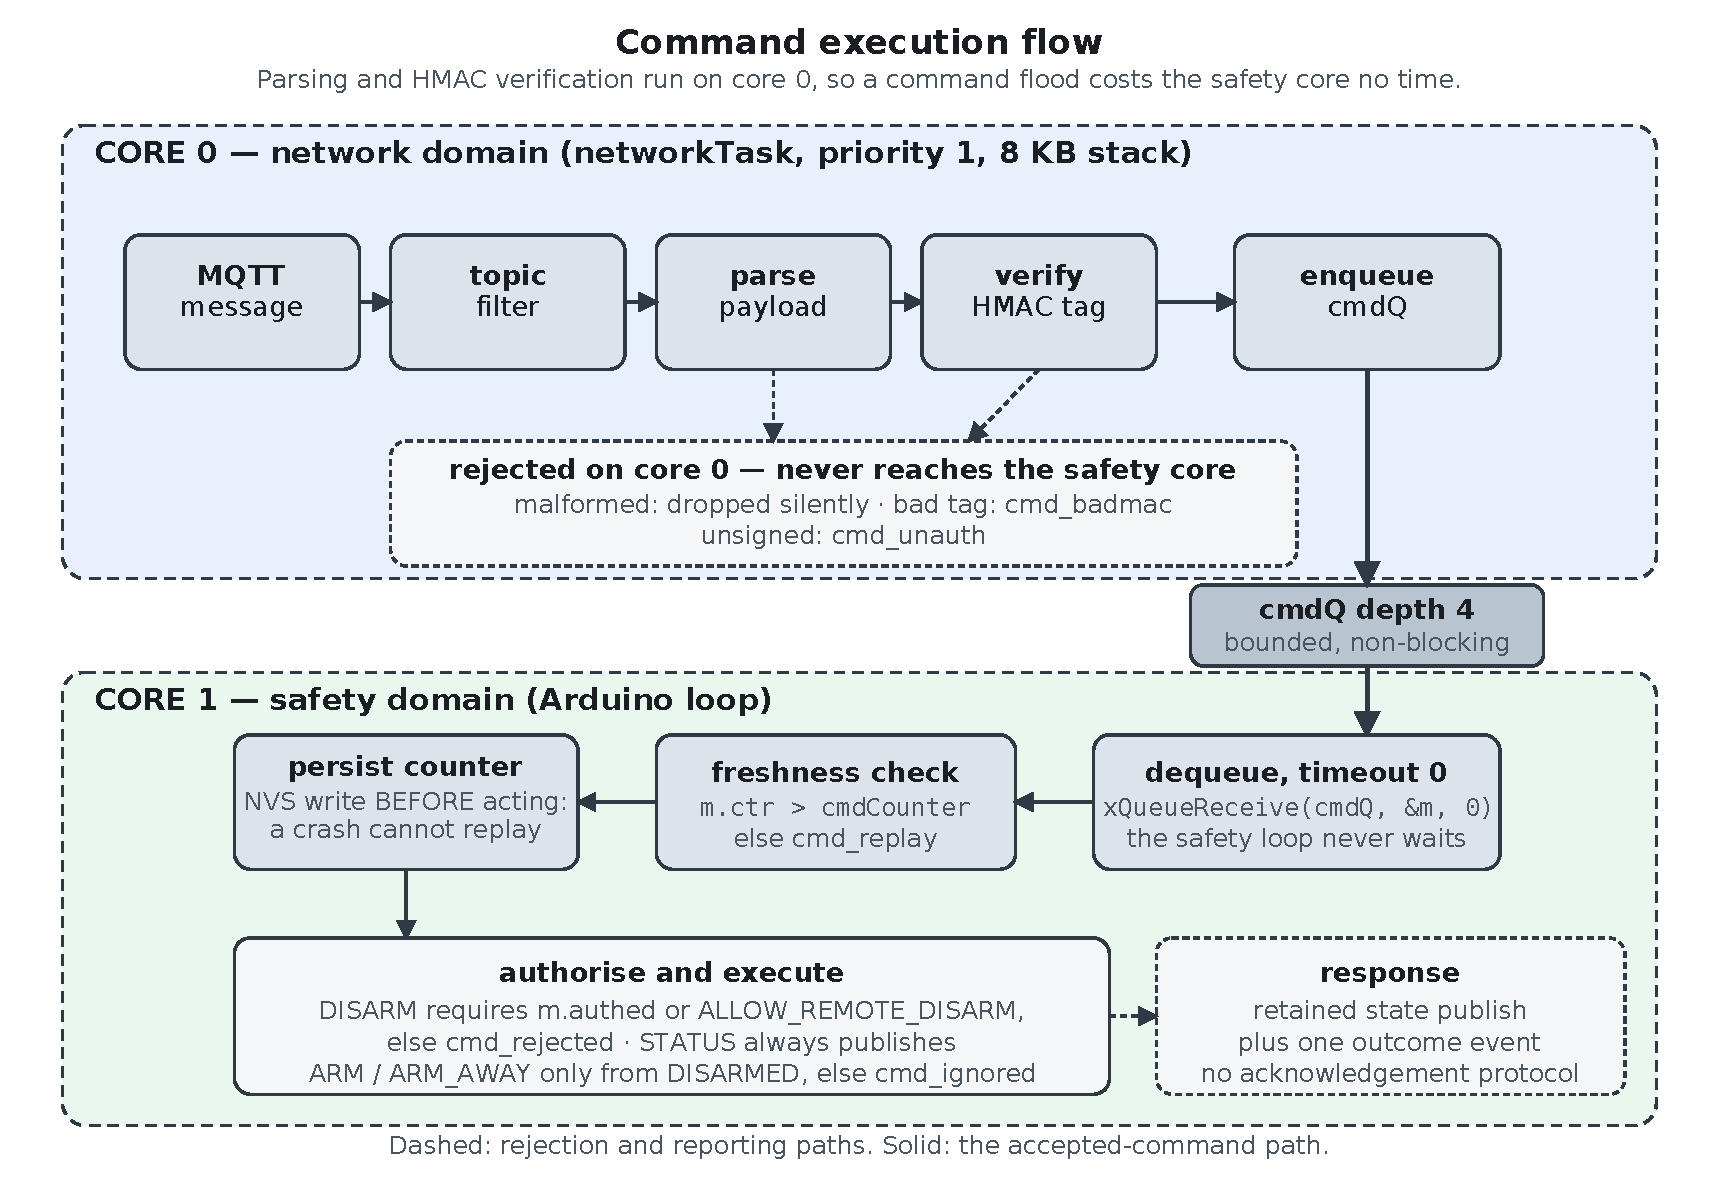
\includegraphics[width=\textwidth]{command_flow.pdf}
\caption[Command execution flow]{Command execution flow. Parsing and verification complete on
core~0; the replay counter is committed to non-volatile storage before the command is acted on.
Rejected commands never reach the safety core.}
\label{fig:cmdflow}
\end{figure}

The ordering is deliberate. All parsing, all cryptographic verification and all rejection happen
on core~0. A malformed, unsigned or incorrectly signed command is discarded there and never
occupies a queue slot. Only a verified command is enqueued, so the safety core's work per
command is bounded and small.

The wire format is deliberately minimal:
\[
\texttt{VERB}:\texttt{CTR}:\mathrm{hex}\bigl(\mathrm{HMAC\text{-}SHA256}(k,\ \texttt{"VERB:CTR"})[0{:}16]\bigr)
\]
A verb, a counter, and a 128-bit truncated tag over both. The tag covers the counter, so an
adversary cannot replay a captured command with a higher counter.

\section{Security architecture}

Three layers are available, and Chapter~\ref{ch:security} reports what each does and does not
contain. Figure~\ref{fig:aclarch} shows the broker-side permissions.

\begin{figure}[htbp]
\centering
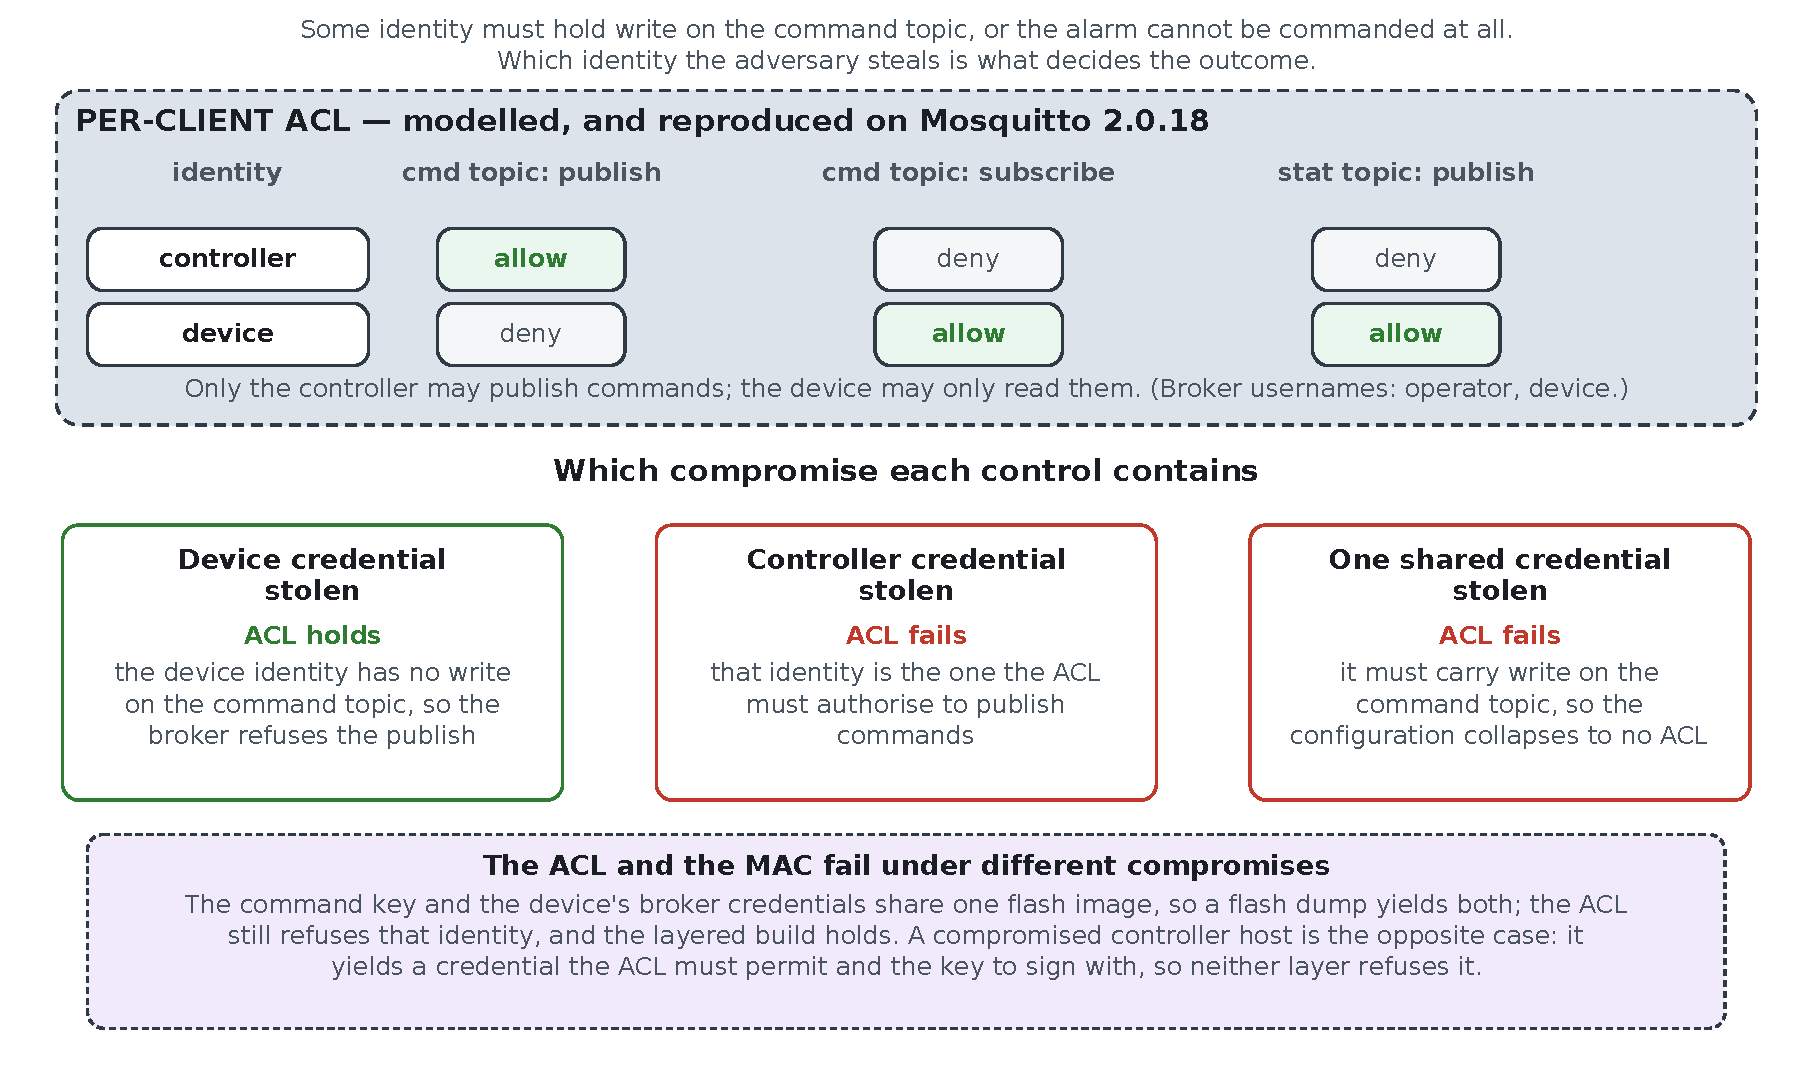
\includegraphics[width=\textwidth]{acl_architecture.pdf}
\caption[Broker access control architecture]{Per-client topic permissions, and which compromise
each control contains. The matrix is both the configuration the ablation models and the
Mosquitto \code{acl\_file} used in the broker experiment.}
\label{fig:aclarch}
\end{figure}

\begin{enumerate}[leftmargin=1.8em,itemsep=5pt]
  \item \textbf{Transport: TLS.} Protects each hop. Does not survive the broker, because the
        broker terminates the connection and re-originates the message.
  \item \textbf{Broker authorisation: per-client credentials and a deny-by-default access
        control list.} The controller identity may publish on the command topic; the device
        identity may only read it. This contains a compromised \emph{device} credential and
        cannot contain a compromised \emph{controller} credential, because the list must permit
        that identity to publish.
  \item \textbf{Application layer: HMAC-SHA256 over a monotonic counter.} Survives any broker
        credential compromise on its own, and falls only when the key itself is compromised.
\end{enumerate}

The counter is persisted to non-volatile storage \emph{before} the command is acted on, not
after. Committing afterwards would leave a window in which a power interruption between action
and commit permits a replay.

\section{Operator and controller interactions}

Three parties exist in the deployed system, and their separation is what the access control list
encodes.

\begin{itemize}[leftmargin=1.6em,itemsep=4pt]
  \item \textbf{The device} subscribes to the command topic and publishes state and events. In
        the broker configuration its username is \code{device}.
  \item \textbf{The controller} — a phone application, Home Assistant or Node-RED — publishes
        commands and reads state. Its username is \code{operator}. It is the identity the access
        control list must authorise to publish, which is why its compromise is scenario~E$'$.
  \item \textbf{The broker} mediates. In the default configuration this is a public test broker;
        the evaluation used a private Mosquitto instance with TLS, per-client credentials and
        the access control list shown in Figure~\ref{fig:aclarch}.
\end{itemize}

\section{What the architecture does not contain}

Stated explicitly, so the diagram is not read as claiming more than it shows.

\begin{itemize}[leftmargin=1.6em,itemsep=4pt]
  \item \textbf{No secure element and no hardware key storage.} The command key is in the flash
        image. This is why a flash dump yields it, and why scenario E exists.
  \item \textbf{No secure boot and no flash encryption.} Both are available on the ESP32 and
        neither is enabled in the artefact studied.
  \item \textbf{No over-the-air update path.} A deployed device would need one; its absence
        removes an attack surface and a capability at the same time.
  \item \textbf{No key rotation or provisioning protocol.} Out of scope, as
        Section~\ref{ch:req} states.
  \item \textbf{No redundant sensing or watchdog escalation beyond the framework default.}
\end{itemize}
